%!TEX TS-program = xelatex
%!TEX encoding = UTF-8 Unicode

\documentclass[12pt]{extarticle}
% extarticle is like article but can handle 8pt, 9pt, 10pt, 11pt, 12pt, 14pt, 17pt, and 20pt text

\def \ititle {Origins of Mind}
 
\def \isubtitle {Lecture 01}
 
\def \iauthor {Stephen A. Butterfill}
\def \iemail{s.butterfill@warwick.ac.uk}
\date{}

%for strikethrough
\usepackage[normalem]{ulem}

\input{$HOME/Documents/submissions/preamble_steve_handout}

%\bibpunct{}{}{,}{s}{}{,}  %use superscript TICS style bib
%remove hanging indent for TICS style bib
%TODO doesnt work
\setlength{\bibhang}{0em}
%\setlength{\bibsep}{0.5em}


%itemize bullet should be dash
\renewcommand{\labelitemi}{$-$}

\begin{document}

\begin{multicols}{3}

\setlength\footnotesep{1em}


\bibliographystyle{newapa} %apalike

%\maketitle
%\tableofcontents




%--------------- 
%--- start paste
\def \ititle {Origins of Mind}
 
\def \isubtitle {Lecture 01}
 
 
 
\
 
 
 
\begin{center}
 
{\Large
 
\textbf{\ititle}: \isubtitle
 
}
 
 
 
\iemail %
 
\end{center}
 
 
 
\section{The Question}
 
\textbf{Question}
How do humans first come to know about---and to knowingly manipulate---objects, causes, words, numbers, colours, actions and minds?
 
‘... ’tis past doubt, that Men have in their Minds several Ideas, such as are those expressed by the words, Whiteness, Hardness, ... and others: It is in the first place to be enquired, How he comes by them?’
\citep[p.\ 104]{Locke:1975qo}
 
‘How does it come about that the development of organic behavior into controlled inquiry brings about the differentiation and cooperation of observational and conceptual operations?’
\citep[p.\ 12]{Dewey:1938yp}
 
‘the fundamental explicandum, is the organism and its propositional attitudes ... Cognitive psychologists accept ... the ... necessity of explaining how organisms come to have the attitudes to propositions that they do.’
\citep[p.\ 198]{Fodor:1975pb}
 
 
 
\section{From Myths to Mechanisms}
 
‘the soul inherently contains the sources of various notions and doctrines which external objects merely rouse up on suitable occasions’
\citep[p.\ 48]{Leibniz:1996bl}
 
‘Men, barely by the Use of their natural Faculties, may attain to all the Knowledge they have, without the help of any innate Impressions; [...]
‘it would be impertinent to suppose, the Ideas of Colours innate in a Creature, to whom God hath given Sight, and a Power to receive them by the Eyes from external Objects’
\citep[p.\ 48]{Locke:1975qo}
 
‘Developmental science [...] has shown that both these views are false’
\citep[p.\ 89]{Spelke:2007hb}.
 
 
 
\section{Davidon's Challenge}
 
‘We have many vocabularies for describing nature when we regard it as mindless, and we have a mentalistic vocabulary for describing thought and intentional action; what we lack is a way of describing what is in between’ \citep[p.\ 11]{Davidson:1999ju}
 
 
 
\section{An Illustration of Davidon's Challenge}
 
\textit{Object permanence}: the ability to know facts about objects you aren't currently perceiving.
 
When do humans first come to know facts about the locations of objects they are not perceiving?
 
\begin{center}
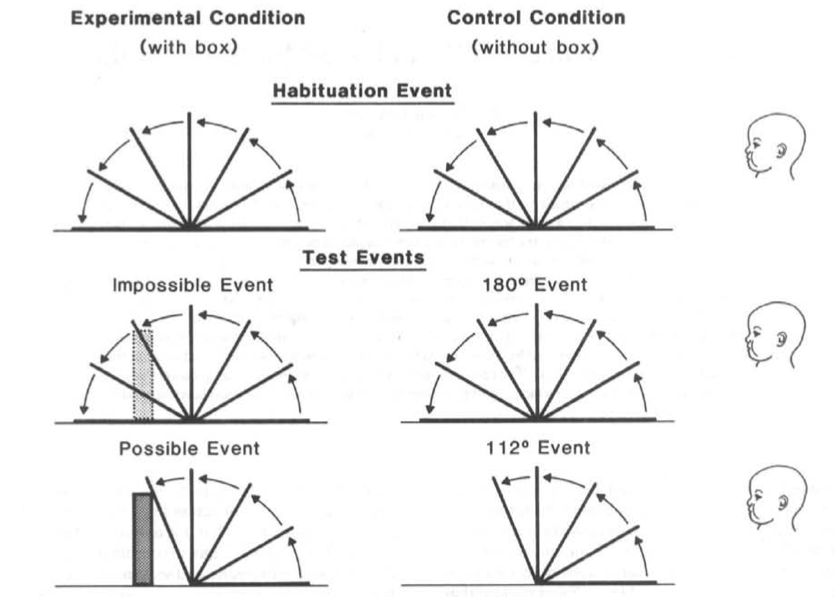
\includegraphics[scale=0.3]{img/baillargeon_1987_fig1.neg.png}
\end{center}
\begin{center} \citealp{baillargeon:1987_object} figure 1 \end{center}
 
\begin{center}
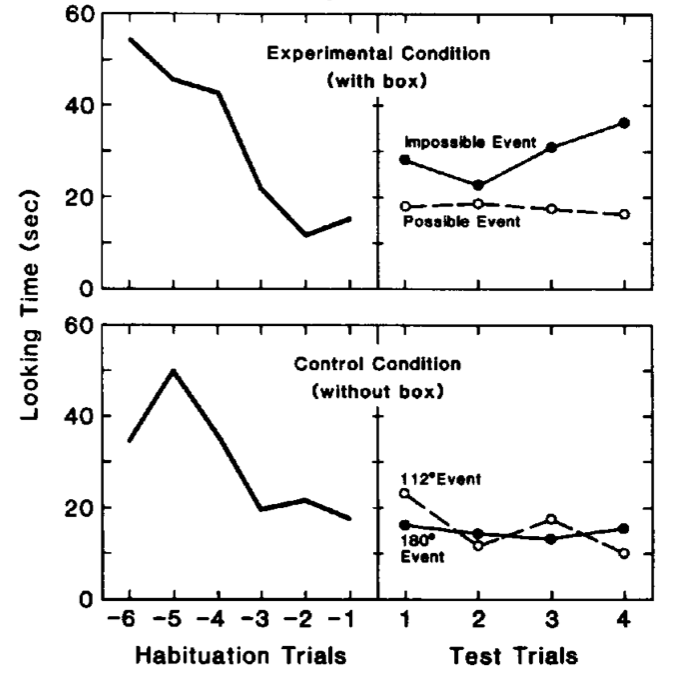
\includegraphics[scale=0.3]{img/baillargeon_1987_fig2.neg.png}
\end{center}
\begin{center} \citealp{baillargeon:1987_object} figure 2 \end{center}
 
‘action demands are not the only cause of failures on occlusion tasks’
\citep[p.\ 291]{shinskey:2012_disappearing}
 
‘violation-of-expectation experiments, using looking-time measures, suggested that infants have object permanence in occlusion conditions; but simplified-search studies confirm that infants fail to reach towards occluded objects, suggesting that infants do not have object permanence in occlusion conditions. This discrepancy, however, is only the tip of the iceberg. Results of studies attempting to measure infants’ cognitive abilities using reaching measures often contradict results gained while using looking-time measures.’ \citep[p.\ 994]{charles:2009_object}
 
‘there are many separable systems of mental representations ... and thus many different kinds of knowledge. ... the task ... is to contribute to the enterprise of finding the distinct systems of mental representation and to understand their development and integration’
\citep[p.\ 1522]{Hood:2000bf}.
 
 
 
\section{Two Breakthroughs}
 
\subsection{A Conjecture}
 
‘humans acquire knowledge at a pace far outstripping that found in any other Recent evidence indicates that interpersonal understanding [...] plays a pivotal role in this achievement.’
\citep[p.\ 40]{Baldwin:2000qq}
 
‘functions traditionally considered hallmarks of individual cognition originated through the need to interact with others ...\ perception, action, and cognition are grounded in social interaction.’
\citep[p.\ 103]{Knoblich:2006bn}
 
Vygotskian Intelligence Hypothesis:
‘the unique aspects of human cognition ... were driven by, or even constituted by, social co-operation.’
\citep[p.\ 1]{Moll:2007gu}
 
‘human cognitive abilities ... [are] built upon social interaction’
\citep{sinigaglia:2008_roots} %*page
  
%--- end paste
%--------------- 
 
\footnotesize 
\bibliography{$HOME/endnote/phd_biblio}

\end{multicols}

\end{document}